%----------------------------------------------------------------------------------------

\documentclass[12pt]{article}
\usepackage[utf8]{inputenc}
\usepackage{graphicx}
\graphicspath{ {Images/} }
 \renewcommand{\familydefault}{\sfdefault}
\usepackage{lmodern}
\usepackage[utf8]{inputenc} % Required for inputting international characters
\usepackage[T1]{fontenc} % Output font encoding for international characters
\usepackage{caption}
\usepackage{subcaption}
\usepackage{mathpazo} % Use the Palatino font by default
\usepackage{hyperref}
\usepackage[table,xcdraw]{xcolor}
\usepackage{float}




\usepackage[a4paper,width=150mm,top=25mm,bottom=25mm]{geometry}

\usepackage{cite}


\begin{document}

%----------------------------------------------------------------------------------------
%	TITLE PAGE
%----------------------------------------------------------------------------------------
%
 \begin{titlepage}
\begin{figure}[h!]
\begin{minipage}[height=2cm]{0.4\linewidth}
    
\includegraphics{ETH_logo}
\end{minipage}
\begin{minipage}[height=2cm, right]{0.2\linewidth}
	\begin{flushright}
    	
\includegraphics[height = 2cm]{D-ERW_logo}
	\end{flushright}
\end{minipage}
\end{figure}


    \begin{center}

    	\Large 
    	Master Thesis Proposal
        \vspace*{1cm}
 
        \Huge
        \textbf{Automated Mapping of Snow Cover on Swiss Glaciers with Sentinel-2: Data Processing and Analysis}
 
        \vspace{0.5cm}
        \Large
        Department of Earth Science D-ERDW\\
        \large
         Institute of Geophysics
 
        \vspace{1.5cm}
 
 		
       \textbf{Lea Geibel}
 
 
        \vspace{2cm}
 		\normalsize
        \textbf{Supervisor}:
        
        \vspace{0.5cm}

       
        Prof. Dr. Daniel Farinotti, Laboratory of Hydraulics, Hydrology and Glaciology VAW, ETH Zürich
        
        \vspace{0.5cm}
        
        Prof. Dr. Hansruedi  Maurer, Exploration and Environmental Geophysics, Department of Earth Science, ETH Zürich 
        
        \vspace{0.5cm}
        Johannes Landmann, Laboratory of Hydraulics, Hydrology and Glaciology VAW, ETH Zürich     
       
        \vspace{2 cm}


        \vspace{0.5cm}

        handed in on 30.01.2019
 
    \end{center}
\end{titlepage}

%----------------------------------------------------------------------------------------
%	DECLARATION PAGE
%----------------------------------------------------------------------------------------


%----------------------------------------------------------------------------------------
%	ABSTRACT PAGE
%----------------------------------------------------------------------------------------

\begin{abstract}
The classification of snow cover on glaciers with optical remote sensing data is challenging but has the potential to greatly improve the availability and quality of data for glacier monitoring. For the Swiss Glaciers, the CRAMPON (Cryospheric Monitoring and Prediction Online) project, is developing an operational modeling tool to nowcast and predict mass balance and runoff to provide a near real-time source of information on their current state and determine the behavior of the glaciers in the future. The melt model of the CRAMPON project needs to be calibrated with information on the current snow cover and the position of the snow line to continuosly provide good results.
\\
\\
Therefore, the first part of this thesis aims to utilize optical Sentinel-2 images to create an algorithm that automatically maps the snow cover on all Swiss glaciers that can then be assimilated into the CRAMPON model. This algorithm will be implemented into a fully automated object-oriented processing framework that performs the necessary pre-processing, scene corrections and the scene classification. Two classifcation algorithms for snow cover mapping on ice by \cite{Rastner2017} and \cite{Naegeli2018} will be implemented for this.
\\
\\
The method will provide a snow cover map and the snow line altitude (SLA) for all Swiss glaciers. In a second part, this output will be validated against a manually derived data set to test the reliability of the method, reveal strengths and weaknesses of the algorithms and determine possible sources for uncertainties.\\
\\
In a third part, a spatio-temporal statistical analysis will be conducted on a test set of glaciers (Rhonegletscher, Griesgletscher, Findelgletscher, Silvrettagletscher, Glacier de la Plaine Morte, Grosser Aletschgletscher) to reveal variations of the SLA and snow cover. 
Furthermore, a comparison with in-field mass balance data from the Swiss Glacier Monitoring Service GLAMOS and runoff data from the glacier catchments will be performed to further validate the method and investigate the correlation with field data.



\end{abstract}

\thispagestyle{empty}
\newpage
%----------------------------------------------------------------------------------------
%	LIST OF CONTENTS/FIGURES/TABLES PAGES
%----------------------------------------------------------------------------------------

\tableofcontents % Prints the main table of contents
\thispagestyle{empty}

\newpage
%----------------------------------------------------------------------------------------
%	THESIS CONTENT - CHAPTERS
%----------------------------------------------------------------------------------------


\setcounter{page}{1}
\section{Introduction}
\subsection{Motivation}
The rapid  retreat of glaciers worldwide is an indicator of climate change and global warming \cite{Barry2006}. Despite one of the world's best glacier monitoring networks with a long tradition in Switzerland, there are still many unkowns about the the dynamics of glaciers and their coupling to the climate. To better quantify the evolution of glaciers and their reponse to external forcings like the climate, mass balance models are widely applied in Glaciology( e.g. \cite{Huss2008}, \cite{Zemp2009}) .
For the Swiss glaciers, the CRAMPON project (Cryospheric Monitoring and Prediction Online) is developing an operational modeling tool to nowcast and predict mass balance and runoff to provide a near real-time source of information on their current state and determine the behavior of the glaciers in the future. \\
\\
The mass balance of a glacier is the sum of how much mass a glacier is gaining e.g. due to precipitation and loosing e.g. due to melting. To determine the mass balance, the amount of snow cover on the glacier and the corresponding snow line altitude (SLA) can provide valuable information.
To improve mass balance nowcasting, the position of the corresponding transient snow line (TSL) can be used for the calibration of melt models. Therefore, information given by the position of the TSL during the summer is employed to constrain the amount of melt by iteratively calibrating a temperature index melt model \cite{Barandun2018}. 
The other use of this information in the CRAMPON project is for an online assimilation of the snow-covered area to enhance the accuracy of estimated melt in the model. \\
\\
With the rapidly increasing availability of free, high-resolution satellite image data with revisiting times within in the range of days (Landsat 7 and 8, Sentinel mission), new possibilities to employ this data in remote sensing applications arise. In this project, Sentinel-2 optical data will be used to capture the varying snow cover of the Swiss Glaciers every 2-3 days, depending on the cloud cover in the areas. Using this approach, we will derive a series of snow cover maps with high temporal resolution as an input for the CRAMPON project.To incorporate this information into a nowcast and mass balance prediction model for a longer term, a mapping algorithm that is eligible for automated processing needs to be found. Therefore, this thesis will aim to develop such an algorithm, implement it into a fully automated programming framwork and validate the results.

\subsection{Spectral Reflectance of Snow and Ice}
The key to successfully map snow on glacier ice is the characteristics of the spectral response of snow in certain wavelength regions of the visible and near-infrared part of the solar spectrum \cite{Koenig2001}.  \\
\\
As shown in Figure \ref{fig:reflectance_ice}, the spectral response of ice and snow is highly varying and depends on many different parameters such as age of snow, water content, grain size and impurities and it is therefore difficult to determine the type of surface cover only by its reflectance.In general, snow has a high reflectance of over 0.9 (this means that 90\% of incoming sun radiation is reflected by it)in the visible (VIS) wavelengths (400 to 700nm) whereas the VIS reflectance of pure ice is around 0.6 \cite{ZengQunzhu1984}. This behavior can be explained by the fact that in the VIS range the reflectance is mostly influenced by impurities on the surface \cite{Warren1980a}.\\
For glacier ice, the reflectance in the far infrared (IR) wavelengths (over 700 nm) decreases significantly, while for ice the decrease is stronger with a steeper slope than for snow. This is due to the effect of the grain size in the middle infrared region, leading to a strong decrease for larger grain sizes \cite{Wiscombe1980}. 
The fact that the reflectance in the near-infrared range is different for ice and snow can be used to distinguish them in optical remote sensing images \cite{Dietz2011}.\\
\begin{figure}
\centering 
    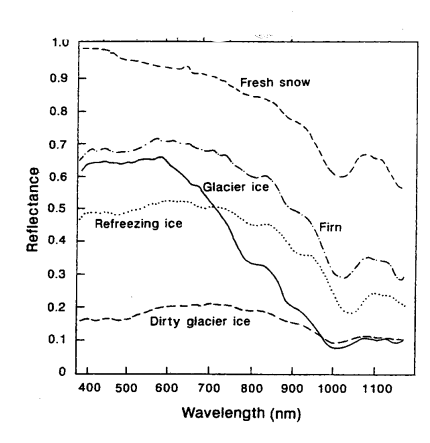
\includegraphics[width=0.6\textwidth]{zeng_et_al__as_modified_by_koenig_spectral_reflectance.png}
    \caption{Spectral reflectances of snow and ice, after \cite{ZengQunzhu1984}, as modified by König, 2001 }
    \label{fig:reflectance_ice}
\end{figure}


\begin{figure}
    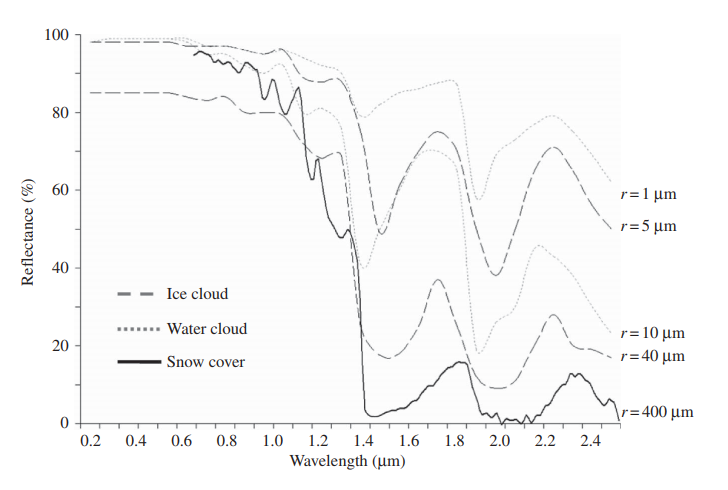
\includegraphics[width=0.8\textwidth]{dozier_et_al_as_modified_byKoenig_et_al_cloud_reflectance.png}
    \caption{Spectral reflectances of snow and clouds, after \cite{Dozier1989}, as modified by \cite{Dietz2011} }
    \label{fig:reflectance_clouds}
\end{figure}
Looking at the spectral reflectance of of snow cover, one point that makes its correct classification difficult is the  differentiation between clouds and snow since they exhibit a very similar spectral behavior in the visible and thermal range. One characteristic that can be used to discriminate between snow and clouds is the grain size of the particles (Figure \ref{fig:reflectance_clouds}). Water droplets and ice particles in clouds have much smaller grain sizes (10 $\mu m$ and 40 $\mu m$) than typical snow grains (400 $\mu m$). This leads to a stronger decrease in reflectance of snow particles in the SWIR than for clouds and can therefore be used to detect cloud cover over snow-covered areas \cite{Dietz2011}. 
\\
\\
With this knowlegde about the spectral characteristics of ice and snow, a mapping algorithm for snow cover on glaciers can be determined.
 \\



\section{Current State of Reseach in ihe Field}
\subsection{General Research on Classification of Snow on Glaciers}
A typical approach for a scene classification such as the one between ice and snow with optical satellite imagery is to employ multispectral thresholding on different bands \cite{Schowengerdt2012}. This approach has been widely applied to discriminate between snow and land surfaces (e.g. \cite{Paul2016}, \cite{Koenig2001} for a review), often using thresholding on simple bands or differential ratios such as the Normalized Difference Snow Index (NDSI), first introduced by \cite{Hall1995}. It employs the characteristic slope between the high VIS and the low shortwave infrared (SWIR) reflectance of snow as a a ratio between those two bands. For Sentinel-2 Data, the spectral Bands 3 and Band 11 are used and the NDSI is defined as $NDSI = \frac{B3-B11}{B3+B11}$.  For the classification of snow, usually a set of fix thresholds are applied, e.g. classifying pixels with an NDSI over 0.2 as snow. 
Many of them have manually been applied successfully to map glacier extents \cite{Paul2016} and some have also been implemented into an automated workflow (e.g. the SNOWMAP algorithm for MODIS, \cite{Hall1995} or the snow scene classification of Sentinel-2 Level 2 A data \cite{SentinelHandbook2015}).\\
 \\
Different approaches to find appropriate band combinations and thresholds are applied. Often, a variety of combinations are tested and a visual or statistical validation determines the ones providing the best results for the area of interest\cite{Rabatel2012}, \cite{Paul2016}. In the recent past, there has been an increasing effort to use machine learning to find the best band combinations and thresholds for an automated scene classification for snow and ice cover mapping(e.g. \cite{Bonev2017} for sea ice mapping or the Sentinel-2 scene classification algorithm \cite{SentinelHandbook2015}).This is possible because generally the contrast between snow and surrounding soil is high enough to discriminate between them with the thresholding approach that can often be automated.\\
\\
In contrast to a general snow classification, the discrimination between snow and ice faces more challenges. Since their spectral reflectances are more similar than that of snow and other soil types, influences like terrain or cloud shadows especially in mountainous terrain often create higher contrasts than the contrast between snow and ice. Therefore, using simple or differential band ratios like the NDSI, that can correct for terrain induced illumination differences only to a small extent are not succesful at mapping snow cover on glaciers \cite{Khan2015}, \cite{Paul2016}.  \\
\\
Even though an automated classification is challenging, the contrast between snow and ice is often visible in single bands like the NIR band, but can still be enhanced by using a multispectral approach.
\cite{Rabatel2012} finds a combination of the green, NIR and SWIR band to yield the best contrast for a manual delineation of the SLA on glaciers in tropical areas. This can be further improved by applying manually adapted thresholds to the NIR and green band \cite{Rabatel2012}, but terrain-shaded areas can still not be mapped correctly. However, no statistical analysis or validation of the method has been conducted, but the approach has been widely applied since then (\cite{Veettil2015},  \cite{Khan2015}).
\\
\\
 Therefore, a careful preprocessing and correction of the images with secondary information such as a DEM becomes crucial for any successful classification of snow on glaciers (\cite{Bippus2011}, \cite{Paul2016}).
\\
 One way to approach this challenge is to apply the best achievable terrain correction with a DEM to account for terrain induced shadows. In this thesis, two recently developed algorithms that are dealing with those challenges for an automated classification of snow cover on glaciers will be implement  into an automated processing framework for Sentinel-2 data and tested in the Swiss Alps.\\
\\
The first method presented by \cite{Rastner2017} relies on a detailed topographic correction and applies the Otsu-algorithm to the NIR band of each glacier to find the individual optimum threshold that maximizes the inter-class variance and minimizes their combined spread. \\
The other algorithm by \cite{Naegeli2018} focuses on the shortwave broadband albedo in a multi-step classification scheme including the glacier geometry and altitude to retrieve the bare-ice area versus snow-covered surfaces.

\subsection{ASMAG Algorithm by \cite{Rastner2017}}
\label{ASMAG}
The 'Automated snow mapping on glaciers' (ASMAG) algorithm (Figure \ref{fig:ASMAG}) that \cite{Rastner2017} developed uses Landsat scenes of the Alps that were processed individually to detect the snow-covered area and the SLA for each scene. For the processing, the required input consists of all Landsat satellite bands, a DEM containing all glaciers and manually-derived glacier outlines.\\
\begin{figure}[H]
\centering
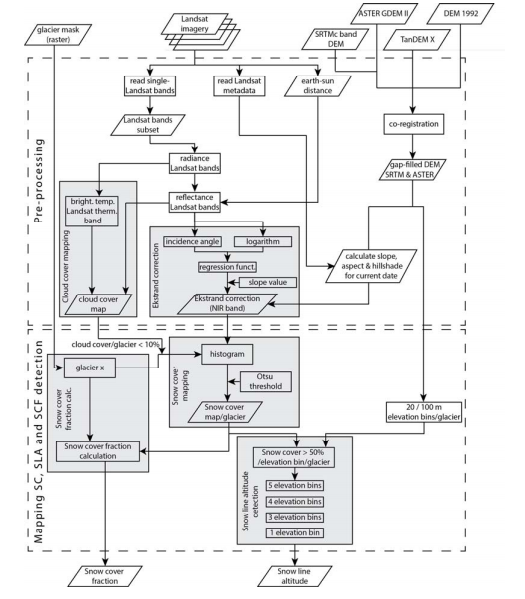
\includegraphics[width=0.9\textwidth]{Rastner_ASMAG}
\caption{Processing flow chart of ASMAG by Rastner, 2017}
\label{fig:ASMAG}
\end{figure}
The Landsat imagery undergoes extensive pre-processing, converting radiance bands to reflectance bands. Then, the sun incidence angle, the slope, aspect and a hill shade of the input DEM is calculated and used to apply an Ekstrand terrain correction to the NIR band reflectance data (details see Section \ref{Ekstrand}, \cite{Ekstrand1996}).\\
From the thermal band, the brightness temperature is derived and applied on bright areas to determine if they are snow (cold) or clouds(warmer). This way, a cloud mask is created that is applied individually to each image and only scenes with less than 10\% cloud cover are processed by the algorithm.\\
\\
The actual thresholding is then performed on the NIR band for each glacier individually using the Otsu-threshold. It assumes that a scene’s histogram is bimodal, having two peaks that correspond to ice and snow and then finds the optimal threshold that maximizes the inter-class variance and minimizes their combined spread. Applying this threshold to the scene gives a direct binary snow cover map of the area. In order to retrieve the snow line altitude in ASMAG, the applied DEM is split into 20 m elevation bins with which the snow-cover map from the previous step is intersected. If the first (lowest) five elevation bins all have a snow cover larger than 50\%, the lowest of these bins is selected as the SLA. If not, the iteration is repeated for the next higher set of five bins. If there are no five continuous bins that meet that criterion throughout the entire glacier, the same test is repeated for four, three, two or one bins to retrieve the SLA.


\subsection{Algorithm by \cite{Naegeli2018}}
\label{Nageli}

In \cite{Naegeli2018}, a method to retrieve the remotely-determined end-of-summer albedo of Swiss glacier ice is described (Figure \ref{fig:naegli}). It uses a mulit-spectral Landsat surface reflectance product and a 30 m resolution DEM as input and the only applied pre-processing is a semi-automated cloud mapping approach to exclude cloud-affected pixels from the classification.In a next step, the discrete narrow-band reflectance is converted to a continuous shortwave broadband albedo. This conversion in general requires knowledge about the spectral response of different snowpacks \cite{Bamber2007}. However, \cite{Naegeli2017} showed that this albedo retrieval approach provides very high accuracy and is suitable for mountain glaciers and can therefore be applied for this method. From the broadband albedo, a multi-step surface type evaluation is performed to discriminate between snow covered areas and bare ice. 

\begin{figure}[H]
\centering
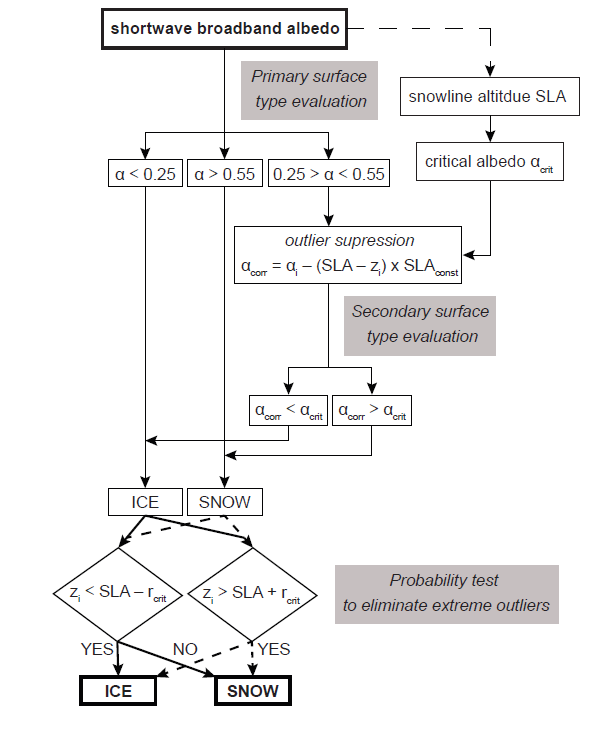
\includegraphics[width=0.7\textwidth]{naegl_algorithm}
\caption{Flow chart of the methodology applied to evaluate the surface type (snow/ice) of every glacier grid cell based on the derived
shortwave broadband albedo, Naegeli, 2018}
\label{fig:naegli}
\end{figure}
First, a primary surface type evaluation is performed based on \cite{Cuffey2010}. With this, every area with an albedo higher than 0.55 is classified as certainly snow and below 0.25 certainly as ice. In the critical albedo range between 0.25 and 0.55, a proxy for the SLA is defined as the altitude that with the strongest albedo change, which is assumed to be the transition between ice and snow. By defining the altitude where the highest slope in the albedo occurs as an estimate for the SLA, the local albedo at this point can be used as a critical value to distinguish ice from snow. All grid cells within the critical albedo range are then reclassified by the critical albedo value and corrected for extreme outliers by their relative altitude compared to the SLA. With this penalty function approach, a high albedo value that is near the glacier terminus will be classified as ice while a low albedo cell high up the glacier will be mapped as snow. This way, the algorithm accounts for deviations in the albedo due to influences like terrain shadows that change the local reflectance. \\
\\


\section{Methodology and Current State of own Research}
In the following section, the necessary methodology for the preprocessing of Sentinel-2 data for an automated algorithm is presented as well as first classification results from a test scene based on the .
\subsection{Sensor and Data}
\subsubsection{Sentinel-2 Data}
Sentinel- 2 is an ESA mission highly complementary to the USGS Landsat 7 and 8 data, that is widely applied for remote sensing applications. It consists of two satellites, Sentinel-2A and 2B, that were launched in 2017. Together, they have a revisiting time of 5 days at the equator with 13 different multispectral imaging (MSI) bands ranging from Visible and Near-Infrared to shortwave infrared with a resolution of 10m to 60 m (see Figure \ref{fig:spectral_bands} for an overview of the bandwidths of the Sentinel-2 bands)

\begin{figure}[H]
\centering
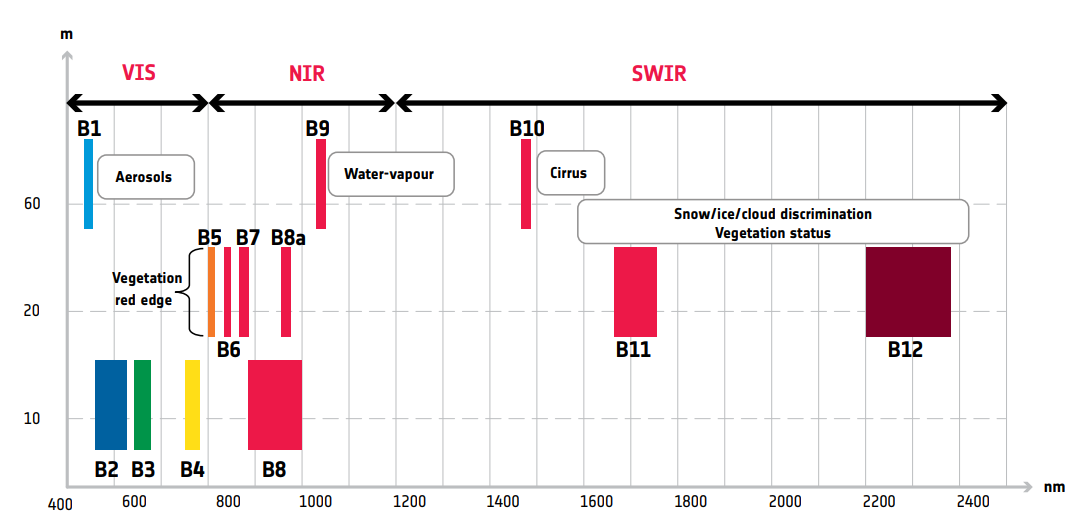
\includegraphics[width=0.9\textwidth]{sentinel_bands}

\caption{Spatial resolution and wavelengths of the Sentinel-2 bands, \cite{ESA_bulletin}}
\label{fig:spectral_bands}
\end{figure}

\subsubsection{Data Retrieval}
 All Sentinel-2 data products can be accessed in the Copernicus Open Access Hub with a free user account. The data is available in 100 $km^2$ x 100 $km^2$ tiles and can be sorted by satellite, region, acquisition date, cloud cover, processing format, and bands. \\
Since this thesis aims to develop an automated processing framework that includes automatic data retrieval, the python API of the open source Python package ‘sentinelsat’ will be used to search the data and metadata for a given date and location, and then download it automatically.

\subsubsection{Processing Levels and Data Formats}
The Sentinel-2 Data is usually delivered in the SENTINEL-SAFE file structure, including image data in JPEG2000 format, quality indicators (e.g. defective pixels mask), auxiliary data and metadata. A detailed description of the file structure and content of the folder can be found in ESAs Technical Guide for Sentinel-2 \cite{SentinelHandbook2015}.\\
The Sentinel-2 Data is currently made available via the Sentinel Hub in two processing levels, Level 1-C and Level 2-A: Level 1-C data gives radiometrically and geometrically corrected Top of Atmosphere (TOA) reflectance per pixel. The Level 2-A product is an orthoimage Bottom-Of-Atmosphere (BOA) corrected reflectance product together with a scene classification map (details in the Sentinel-2 Technical Guide \cite{SentinelHandbook2015}). In the past the Level 1-C data had to be processed manually with the Sen2Cor module \cite{Issue2018} but since 2018, Level 2-A data is also made systematically available via the Copernicus Hub.

\subsection{Preprocessing}
\label{Methodology}
For familiarization with the Sentinel-2 imagery and possible ways to process them with Python, a test set of Level 1-C and Level 2-A products was manually downloaded to assess the quality of the images and their different processing levels. From this it can be determined what pre-processing steps will be necessary for a succesful automated scene classification. In \ref{fig:workflow}, the workflow of the framework that is aimed to be developed is shown with a focus on the preprocessing steps.

\subsubsection{Glacier Mask}
In a first step, the outlines of the glaciers need to be extracted so the algorithm later does not map any snow cover or snow patches that are not on the glaciers. That is done by applying the newest manually derived glacier mask of the Swiss Glacier Inventory SGI from 2018. Despite the recent aquisition date, the SGI 2018 mask classifies many parts as glacier that on the Sentinel-2 satellite images appear not to be part of the ice or snow-covered part of the glacier (left side of Figure \ref{fig:glacier_mask}). This is probably due to shadows or debris cover on the sides of the glaciers. Since those dark sides would significantly reduce the accuracy of our algorithm, a second classification, based on the glacier mapping algorithm by  \cite{Paul2016} for the Swiss alps for Sentinel-2 Data is performed. It classifies a pixel as part of the glacier when it meets the four following criteria:
\begin{enumerate}
 \item $NDSI \geq	 0.20$
 \item $0 \leq MSI4/MSI11 \leq 2$
 \item $MSI2/MSI4 \leq 1.20$
 \item $4.	0 \leq MSI8/MSI11 \leq 1$
\end{enumerate}

The left side of Figure \ref{fig:glacier_mask} shows the SGI glacier mask applied to a scene of Level 1-C data on Rhone Glacier in the NIR Band 08 where the darker sides are still visible. On the right side of Figure \ref{fig:glacier_mask}, the result after the applied thresholding is shown, where the darker sides have successfully been removed. 
However, since this thresholding will automatically exclude all shaded areas, the terrain correction needs to be applied first before this thresholding is performed.

\begin{figure}[t]
\centering
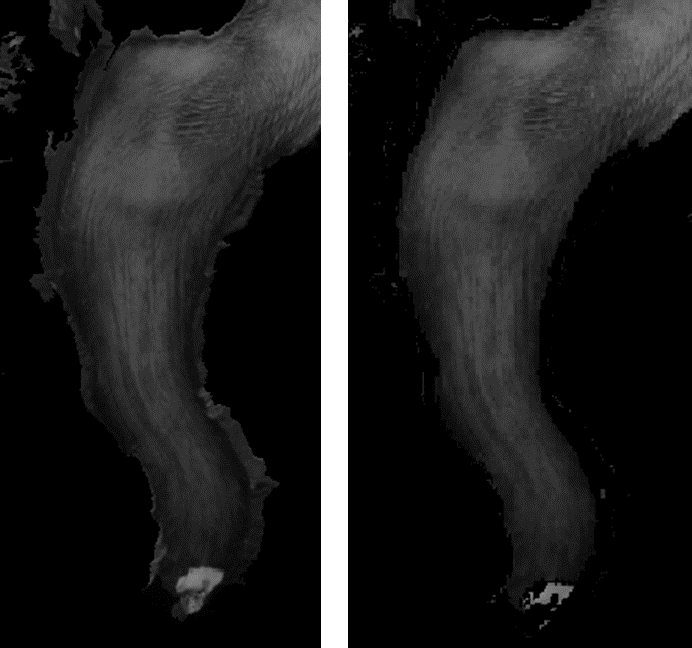
\includegraphics[width=0.7\textwidth]{glacier_mask}
\caption{left: SGI 2018 Glacier mask applied to tongue of Rhone Glacier, right: Dark side areas of Glacier removed with tresholding after \cite{Paul2016}}
\label{fig:glacier_mask}
\end{figure}


\subsubsection{Terrain Correction}
\label{Ekstrand}
Since the study site, the Swiss glaciers, is located in very steep terrain, the scenes are heavily affected by shadows, producing very dark areas that can’t be accounted for by simply using band ratios for classification. Thus, a careful topographic correction will be key to obtain a successful scene classification. \\
In theory, topographically corrected Sentinel-2 images are available with the Level-2A data. However, the details of this correction are unclear and the information provided in the Sentinel-2 Handbook (\cite{SentinelHandbook2015}) are not up-to-date. It describes that the Level 2-A data are obtained manually by the user with the Sen2Cor processing package that performs atmospheric correction from Top-Atmosphere (TOA) to Bottom-of-Atmosphere (BOA) and an optional topographic correction. Those are based on the 90m Shuttle Radar Topographic Mission (SRTM) Digital Elevation Database from the Consortium for Spatial Information of the Consultative Group for International Agricultural Research (CGIAR-CSI) or the commercial 90m Digital Terrain Elevation Data DTED-1 Format from PlanetDEM (Sen2Cor Handbook, \cite{Issue2018}). Since 2018, the Level 2-A data were systematically made available on the Copernicus Platform, but the product description has not changed, suggesting that the Level 2-A data that can be downloaded are atmospherically, though not topographically, corrected. However, when looking at the data in mountainous terrain, it can be seen that some kind of correction has been performed on the shaded areas, but the results are do not display any improvement of the information content (see Figure \ref{fig:RGB_1C} and Figure \ref{fig:RGB_2A} for a comparison of Level 1-C and Level 2-C  products). \cite{Paul2016} also noted that the internal terrain correction for Sentinel-2 data was unsatisfactory for steep terrain. \\
\begin{figure}[t]
\centering 
  \begin{subfigure}[height=7cm]{0.45\textwidth}
    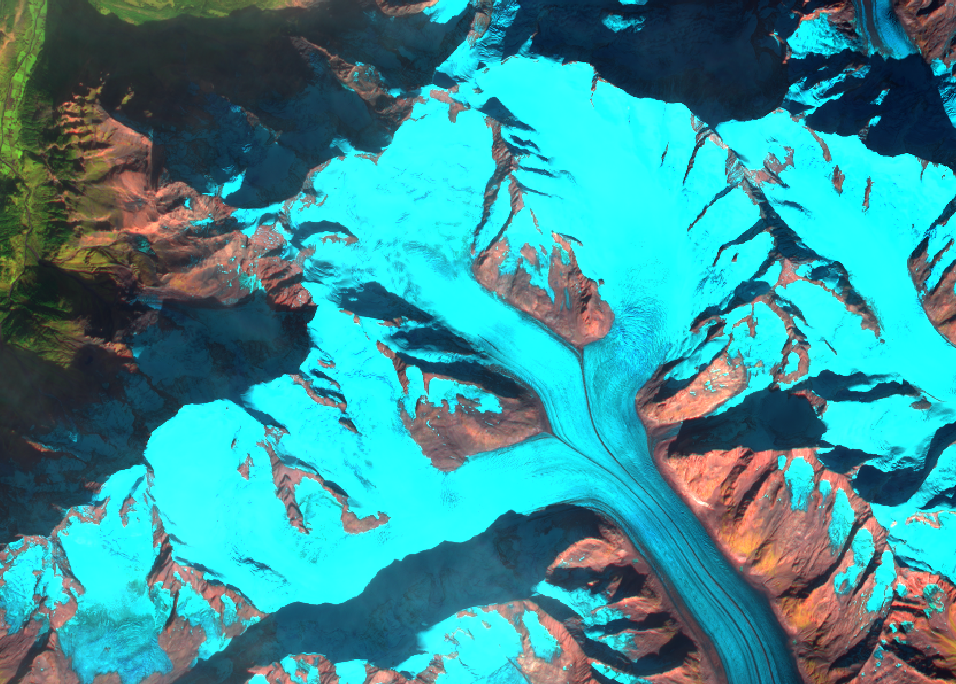
\includegraphics[width=\textwidth]{RGB_1C}
	\caption{RGB composite of green, NIR and SWIR bands of Level 1-C images. Terrain shadows on the north slopes appear very dark}
		\label{fig:RGB_1C}

	\end{subfigure}
	\hspace{0.5cm}
  	\begin{subfigure}[height=7cm]{0.45\textwidth}
    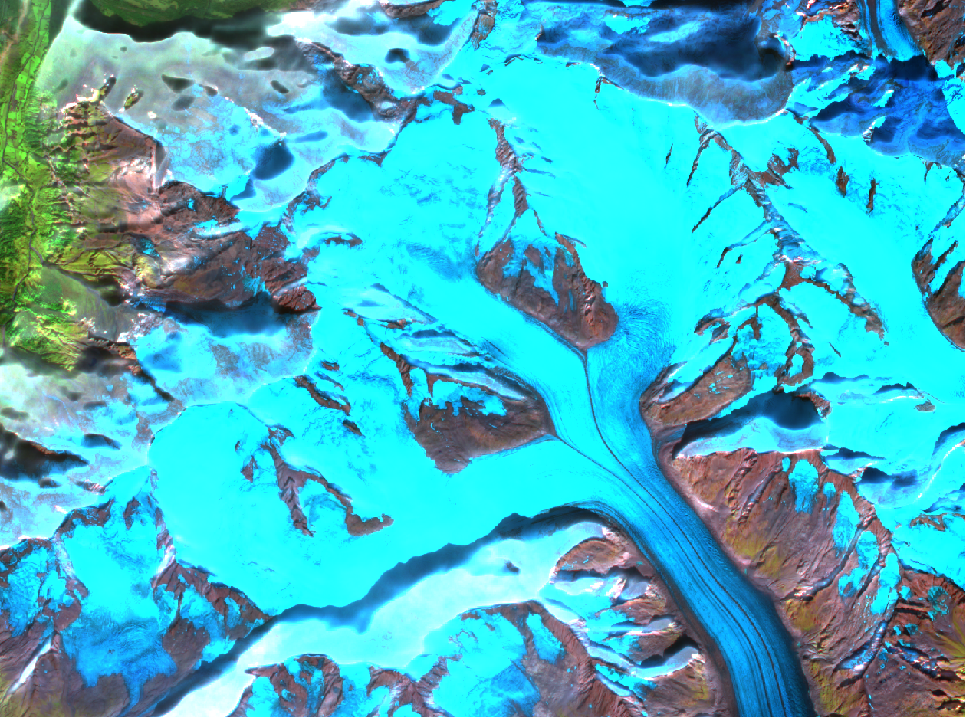
\includegraphics[width=\textwidth]{RGB_2A}
	\caption{RGB composite of green, NIR and SWIR bands of Level 2-A images. Terrain shadows are corrected but result in a loss of information}
			\label{fig:RGB_2A}
	\end{subfigure}
\end{figure}
Therefore, we will use the uncorrected Level 1-C data for our algorithm and perform our own topographic correction. After \cite{Bippus2011}, the best terrain correction for mountainous areas is the Ekstrand correction (\cite{Ekstrand1996})that is widely used in pre-processing in applications for snow-ice mapping (\cite{Paul2016} and the ASMAG algorithm by \cite{Rastner2017}). \\
\\
The Ekstrand correction is based on the solar illumination data of the acquisition date that is available in the Sentinel-2 metadata and aspect, slope and hillshade data derived from a DEM. For this application, the swissALTI 3D DEM with a 10m resolution will be used. The corrected radiance of the horizontal surface is calculated as \\

\begin{equation}
	L_{horizontal} = L_{inclinced}\cdot(\frac{cos(\theta_z)}{cos(i)})^{cos(i)\cdot k}
\end{equation}
where\\
$L_{horizontal}=$ reflectance of the horizontal surface,\\
$L_{inclinced}=$ recflectance of the inclined surface,\\
$\theta_z=$ solar zenith angle,\\
	 $i =$ solar illumination angle derived from slope and aspect maps of DEM as\\
\\
 $cos(i) = cos(e) \cdot cos(\theta_z) + sin(e) \cdot sin(\theta_z) \cdot cos(\phi_s-\phi_a)$\\
	 \\
	 where \\
	 $e =$ surface normal zenith or terrain slope, 
	 \\$\phi_s = $ solar azimuth angle,
	 \\ $\phi_a=$surface aspect/slope angle,
	  \\$k=$ Minneart constant\\
\\
The Minneart constant k is obtained by linear regression of the logarithmic equation (Ekstrand 1995)

\begin{equation}
log(L_{horizontal}) = log (L_{inclinced}) + k \cdot cos(i)\cdot log (\frac{cos(\theta_z)}{cos(i)})
\end{equation}

 Typically a global k-value is used for each scene. However, the Ekstrand correction has not yet been applied to the Sentinel-2 Level 1-C data, so it is still open how the result looks like. Even though it has been indicated that the Ekstrand correction provides the best results in steep alpine terrain \cite{Bippus2011}, it can still be improved further if it should not yield satisfying results.
Normally a global k-value is used for each scene, but an approach by \cite{Lu2008} offers a pixel-based inversion method for the k-value for further improvement of the results if this reveals to be necessary.
 


\subsubsection{Cloud Mask}
In a next step, a suitable cloud detection algorithm needs to be found. Since the Swiss Alps are often affected by cloud cover that is opaque for optical sensors, a correct classification of clouds over the glaciers is crucial in order to obtain a correct snow cover map. This is a challenging step since clouds and snow are very difficult to distinguish in the optical spectrum and therefore many available cloud mapping schemes widely overestimate cloud cover on snowy areas \cite{Koenig2001}, \cite{Coluzzi2018}. \\
\\
In a first approach, the cloud mask delivered with the Sentinel data on a 60 m grid was used. It is based on a threshold applied to the blue B2 band and then the SWIR bands B11 and B12 to take advantage of the differences in the spectral response of snow and clouds as described in the introduction (for details on the thresholding see \cite{SentinelHandbook2015}). On a test scene of Grosser Aletschgletscher from October 2018, this cloud map displayed numerous shortcomings: In the Alpine areas, the algorithm misclassifies large cloud-free areas both over snow and soil as clouds (Figure \ref{fig:cloud_mask}, top). \cite{Coluzzi2018} found similar problems in their study and suggested using this cloud mask with precaution especially in Alpine environments.\\
Another approach that was investigated is to use the scene classification that is provided with the Level-2A products and extract a cloud mask from the scenes that got classified as either “Cloud Medium Probability,” “Cloud High Probability” or “Thin Cirrus” (Figure \ref{fig:cloud_mask}, bottom).  From a visual inspection, the correct classification of clouds in this scene is significantly higher than in the Sentinel-2 cloud mask. Therefore, this cloud mask is used for all further preliminary applications.
\begin{figure}[h]
\centering 
  \begin{subfigure}[height=7cm]{0.45\textwidth}
    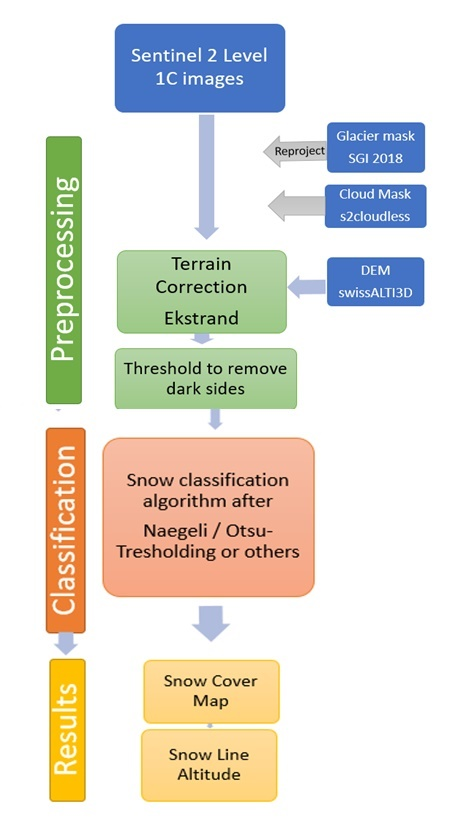
\includegraphics[width=\textwidth]{workflow}
	\caption{Workflow of the automated snow-classification algorithm}
		\label{fig:workflow}

	\end{subfigure}
	\hspace{0.5cm}
  	\begin{subfigure}[height=7cm]{0.45\textwidth}
    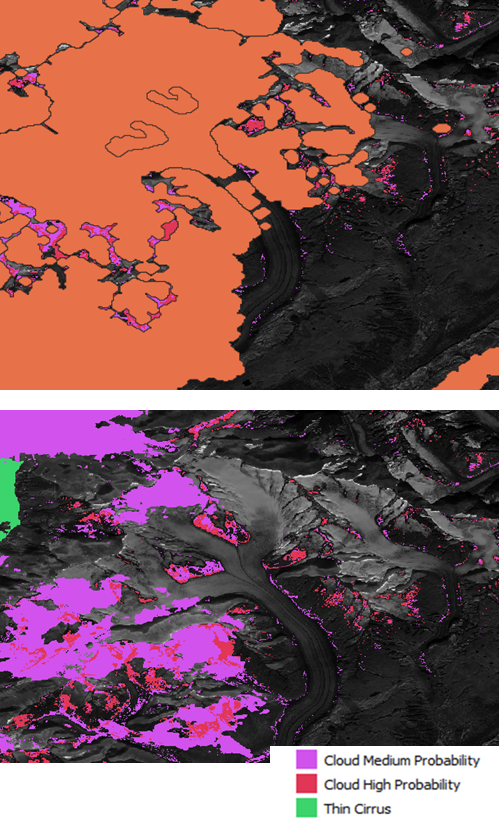
\includegraphics[width=\textwidth]{cloud_mask}
	\caption{Top: Sentinel-2 cloud mask, bottom: cloud mask based on Sentinel-2 scene classification}
			\label{fig:cloud_mask}
	\end{subfigure}
  \caption{Workflow and Cloud Mask}
  \label{fig:workflow_and_cloud_mask}
\end{figure}
However, since those two approaches do still have a large misclassification rate of clouds over snow, other options must be explored. Sentinel Hub itself recognized the need for a good cloud classification algorithm and developed the machine learning based algorithm s2cloudless that performs significantly better than all other approaches, especially on snow \cite{s2cloudless}. A python package to use with Sentinel-2 data containing the algorithm was released recently. During the proposal phase, the package still had some compatibility problems with the the used setup that could not be resolved so far. Thus, the cloud mask based on the Level-2A scene classification was used for the tests, but for the final programming framework, it is aimed to employ the s2cloudless for the best possible performance. \\
\\
Another point that needs to be considered is the maximum cloud cover on a scene that can still be used for a successful classification. In general, a threshold-based method can be applied to any arbitrarily small, cloud-free glacier part and therefore generate useful information on that part. However, when the algorithms become more complex and employ the glacier geometry such as the approach  by \cite{Naegeli2018}, it becomes more and more challenging to produce meaningful results. The same applies for the Ostu-threshold-based ASMAG-algorithm that always assumes a bimodal snow-ice histogram which e.g. with a cloud cover over the entire snowy part of a glacier, leaving only bare ice, will lead to misclassification. Therefore, a certain limit to only include scenes with a lower cloud cover over each glacier must be found once the different algorithms are implemented depending on their individual performance.


\subsubsection{Alternative Approaches for Preprocessing}
Since most of these preprocessing steps have been succesfully applied for Sentinel-2 data \cite{Paul2016}, the results should be a good base for a succesful automated classification. However, if the processing shows not to provide the expected results over the entire Swiss Alps, alternative methods to adress the shadowed areas might have to be explored.\\
Besides approaches such as pixel-based methods for the k-value for a better terrain correction, another possibility would be to extract the shaded areas of the image based on the histogram and do a separate evaluation of the shadow-free and shaded areas. However, it is not yet clear if such an approach will be necessary and will therefore not be further discussed in this proposal.

\subsection{Testing of Algorithms}
\subsection{Results}
After the preprocessing, the actual snow classification is performed on the scene. Since we did not yet employ a DEM in the preliminary work, no manual terrain correction could be performed and no information about the SLA could be derived yet.\\
We used a scene of Level-2A images from October 17th, 2018 of Grosser Aletschgletscher (Figure \ref{fig:aletsch_raw}) for some testing of the approaches of the different algorithms presented in Sections \ref{ASMAG} and \ref{Nageli}. The cloud mask is based on the Level 2-A scene classification, the glacier mask is a combination of the SGI 2018 mask combined with the multispectral thresholding by \cite{Paul2016}. The resulting preprocessed scene on the NIR band is shown in Figure \ref{fig:aletsch_masks}. \\
\\
Firstly, the Otsu-thresholding as used in the ASMAG algorithm was applied to the NIR band (Band 08) to produce a snow cover map (Figure \ref{fig:aletsch_otsu}). To avoid problems with the Otsu-algorithm and small glacier parts, the algorithm was applied to the entire scene.
Secondly, the narrow-to-broadband conversion as suggested by \cite{Naegeli2017} based on the method of [Knap et al., 2016] was performed on band 08 and band 03 to obtain an albedo map with:\\
\begin{equation}
\alpha_{Knap} = 0.726 \cdot b_3 - 0.322 \cdot b_3^2 -0.015 \cdot b_8 + 0.581 \cdot b_8^2
\end{equation}
On this shortwave albedo, the thresholds that discriminate between certainly ice (<0.25) and certainly snow (>0.55) were applied to create a map (Figure \ref{fig:aletsch_naegeli})that represents the snow cover (white) and the area on which the secondary surface type evaluation as described above, will be performed (grey). However, since no DEM was used yet, we could not derive the estimate of the SLA and proceed with the classification.\\
\\
 \begin{figure*}[h]
 \centering
       \begin{subfigure}[height=3cm]{0.475\textwidth}
            \centering
            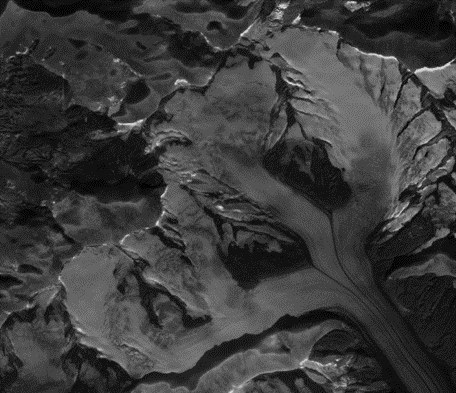
\includegraphics[width=\textwidth]{grosse_aletsch}
            \caption{\small NIR band B08}   
            \label{fig:aletsch_raw}
        \end{subfigure}
        \hfill
        \begin{subfigure}[height=3cm]{0.475\textwidth}  
            \centering 
            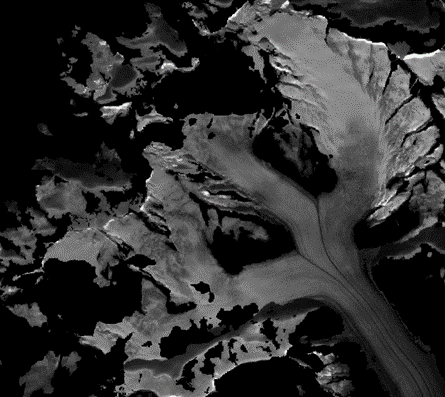
\includegraphics[width=\textwidth]{Altesch_masks}
            \caption{\small Applied glacier and cloud mask}   
            \label{fig:aletsch_masks}
        \end{subfigure}
        %\vskip\baselineskip
       % \medskip
        \begin{subfigure}[height=3cm]{0.475\textwidth}   
            \centering 
            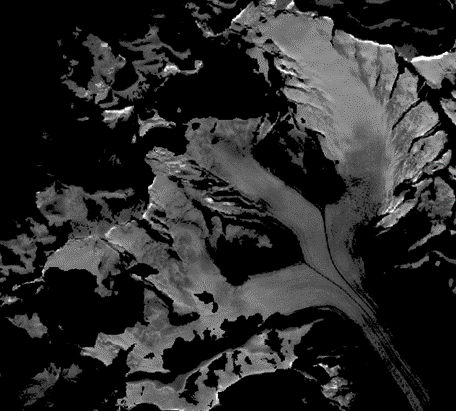
\includegraphics[width=\textwidth]{altesch_otsu}
            \caption{ Snow covered area as classified by Otsu-threshold}   
            \label{fig:aletsch_otsu}
        \end{subfigure}
        \hspace{0.5cm}
        \begin{subfigure}[height=3cm]{0.475\textwidth}   
           \centering 
            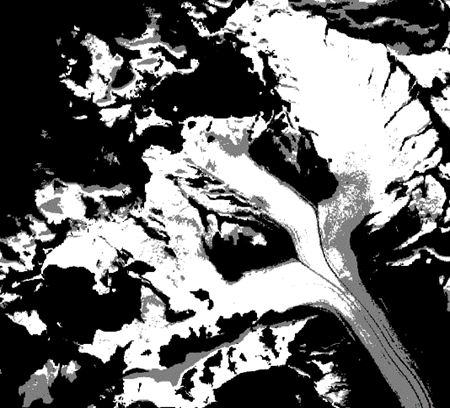
\includegraphics[width=\textwidth]{altesch_naegeli}
            \caption{\small Snow covered (white) and ambiguous area (grey) after \cite{Naegeli2018}}  
           \label{fig:aletsch_naegeli}
       \end{subfigure}
        
        \caption{\small Test scene on Grosser Aletschgletscher, with the applied preprocessing steps and a scene classification for snow after \cite{Rastner2017} and \cite{Naegeli2017}} 
        \label{fig:aletsch}
\end{figure*}
From a visual inspection, the scene shows a rather “patchy” snow cover and contains a mixture of fresh snow and ice areas as well as firn while the tongue of the glacier is bare ice. This feature of the patchy snow cover is a major challenge in the proper classification of snow on glaciers.  Even with the bare eye it is often challenging to give an accurate estimate of the SLA since it is rather a gradual transition zone than a sharp line. \\
\\
Several characteristics can be noted by visually inspecting the results;
The applied Otsu-algorithm performs a first-guess snow cover map for this scene and it classifies 
60.3 \% of the glacier area as snow covered.
The histogram (Figure \ref{fig:histogram}) shows a bimodal distribution, with two peaks representing snow and ice. The Otsu-threshold is calculated as 0.33. However, when comparing the snow-cover map with the NIR band, the threshold seems to be chosen too low, resulting in an overestimation of the snow-covered area, espeially in the lower parts of the image. It can also be seen that many of the areas in the shadow on the north side of the ridgeline are classified as ice on the map even though they are more likely to be snow-covered. This again stresses that the Level 2-A data is not appropriate for a successful classification and a more robust terrain correction is required. \\
\begin{figure}[h]
\centering
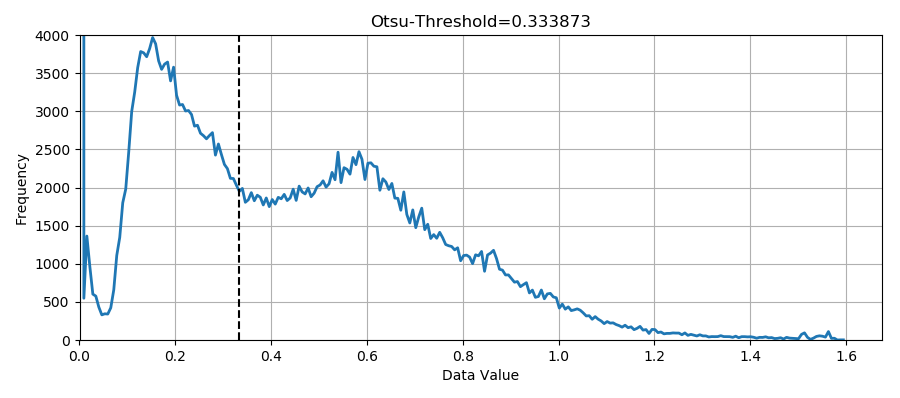
\includegraphics[width=\textwidth]{histogram_otsu_fiescher}
\caption{Histogram of NIR Band over Grosse Aletschgletscher with retrieved Otsu-Threshold}
\label{fig:histogram}
\end{figure}


For the primary surface type evaluation based on the albedo after \cite{Naegeli2018},the area classified as certainly snow (white) is 50.6 \% and the ambiguous area (grey) is 22.3 \%  of the glacier area in this scene (Figure \ref{fig:aletsch_naegeli}).\\
\\
The albedo approach classifies a smaller area than the Otsu-algorithm as certainly snow. Since most of the ambiguous range (grey) is in the higher area of the glacier, the penalty function approach would most likely result in a classification of those as snow, which is correct for many places but also some bare ice areas will be misclassified with this method, leading to a general overestimation of the snow covered area for this scene. The ambiguous range is quite high but without employing a DEM, no further determination of the final snow cover map can be given.

\subsubsection{Discussion of potential shortcomings}
For the ASMAG algorithm by \cite{Rastner2017}, one strong limitation occurs when applying it to all Swiss glaciers. The presence of very many very small glaciers (smaller than 0.5 $km^2$) that are often either completely snow-covered or completely snow-free and that the Swiss Alps posses over 1000 of, are problematic when the Otsu-Thresholding is used. Since the Otsu-Algorithm will always assume a bimodal histogram for each glacier, also the completely snow-covered or snow-free ones, this method will fail to correctly map the snow cover of those glaciers. 

For the method presented by \cite{Naegeli2018}, the penalty function approach for higher elevations will always force the snow map to have a bare ice glacier tongue and a continuous snow cover higher up. In reality the Swiss glaciers often have a rather patchy snow cover and show bare ice areas even higher up the glacier. However, the penalty function in this algorithm with the outlier suppression would classify everything above a certain altitude as snow and therefore not yield a good representation of this natural characteristic. It therefore has to be investigated how much this feature of the method influences the overall accuracy of the snow cover map.

\newpage
\section{Goal of the Thesis}
The thesis will consist of three parts. The goal of the first part is to implement the workflow presented in Figure \ref{fig:workflow} into an automated object-oriented programming framework in python. In a second step, the results should be validated against manually classified scenes via a statistical analysis
The third part of the thesis will be an analysis focusing on the spatio-temporal variability of the snow cover and snow line altitude. \\


\subsection{Part 1: Creating an Automated Object-Oriented Programming Framework}
The goal of the first part of the thesis is to create a fully-automated programming framework in Python. The requirements are that the code is set up in an object-oriented manner that can easily be adapted to work with different inputs and be incoporated in various applications. The code will be able to\\
\begin{enumerate}
\item Download and pre-process the Sentinel-2 images based on cloud cover, terrain corrections, etc. for all Swiss Glaciers as described in the Methodology Section \ref{Methodology}
\item Retrieve a snow cover map and the snow line altitude by applying the algorithms presented by Rastner and Naegeli and possible improvements to these methods
\end{enumerate}

The output will be a binary snow cover map and maps of the snow line altitude for the Swiss Alps. The goal is to implement several different algorithms to be able to evaluate their individual performances.


\subsection{Part 2: Validation of the Algorithms}
In the second part, the obtained snow cover maps will be validated against a manually retrieved data set of the snow cover on the Swiss Glaciers. The validation data set needs to represent the variety of all Swiss glacier while not over- or under-representing any characteristics, i.e. be statisticaly relevant. For this, data for the years of 2016-2018 between the months of May and October will be evaluated to create a wide temporal range and a randomly chosen data set out of all Swiss glaciers to cover a large spatial variety. \\
\\
Since the SLA is a secondary product derived from the snow cover map, the validation of the latter needs to be prioritized. However, a validation of the derived SLA will still be conducted to evaluate the quality of the method to derive the SLA from the snow cover map, e.g. the one presented in the ASMAG algorithm by \cite{Rastner2017}. With those two steps, the strengths and weaknesses of each of the implemented algorithm can be revealed and uncertainties in each  part of the processing workflow determined. Thus, we can find the algorithm that exhibits the best performance for the automated classification of snow cover on the Swiss glaciers. 

\subsection{Part 3: Analysis of Spatio-Temporal Variability of the Snow Cover}
With the retrieved data sets, an extensive spatio-temporal analysis of the snow cover of the Swiss glaciers will be performed. A general spatial analysis will reveal patterns of how the snow cover is distributed over the entire Swiss alps as well as e.g. on the North- and South-slope of individual glaciers.  A temporal analysis will give information about how stable those patterns are, show how they change throughout the summer and between years. For the time series analysis the focus will lie on a set of 7 representative glaciers in the Swiss Alps consisting of Rhonegletscher, Griesgletscher, Findelgletscher, Silvrettagletscher, Glacier de la Plaine Morte and Grosse Aletschgletscher.\\
\\
Furthermore, the obtained SLA time series can be compared to observations that are avilable with a high temporal resolution from the dense monitoring network in the Swiss Alps. It has been shown that the SLA can be correlated to the mass balance on glaciers \cite{Oestrem1973}, \cite{Young1981}, \cite{Hock2007}, \cite{Barandun2018}. 
To investigate this relation for the Swiss Alps, the mass balance data of the Glacier Monitoring Network in Switzerland (GLAMOS) that are collected on a set of Swiss glaciers will be employed. With this information, the correlation between the retrieved remote sensing SLA data and the measured mass balance GLAMOS data for the test set of glaciers will be investigated. Furthermore, temporal variations troughout one (hydrological) year and the variations between different years can be revealed in this analysis. \\
\\
Another measure that has been shown to correlate with the snow cover and the SLA is the glacier runoff. Typically a higher SLA and therefore a lower snow cover results in a lower surface albedo on the glacier, leading to more melting on the glacier and a higher runoff of the glacier \cite{Konovalov1994},\cite{Engelhardt2014}. The Federal Office of the Environment (FOEN) closely monitors the glacier runoff in Switzerland with a dense network. For the test set, the catchments of Rhonegletscher, Griesgletscher, Grosser Aletschgletscher and Glacier de la Plaine Morte have measurement stations available directly at the outflow of the glaciers, allowing a direct comparison. For Griesgletscher, Findelgletscher and Silvrettagletscher the closest stations are further down in the valleys and might therefore also be influnced by other inflows sources. 

 The sum of all measured runoff data of all stations  available for each glacier can then be compared to the  time series of snow cover maps retrieved in this thesis. In the comparison, their correlation will be investigated and a spatio-temporal analysis of the available data will be performed similar to the GLAMOS mass balance data.
  
\section{Timeplan}
\begin{table}[H]
\begin{tabular}{|l|l|}
\hline
Time Schedule Master Thesis: Total 28 weeks (6 Months)                                                                                                                                                                                                                                                                                                                                         & Date /Duration                                                                                     \\ \hline
\cellcolor[HTML]{656565}Start of the Thesis                                                                                                                                                                                                                                                                                                                                                    & 18.02.2019                                                                                         \\ \hline
\rowcolor[HTML]{C0C0C0} 
\textbf{1. Part: Implementation of the algorithm (3 months)}                                                                                                                                                                                                                                                                                                                                   & {\color[HTML]{000000} \begin{tabular}[c]{@{}l@{}}Total for part 1: \\ $\sim$13 weeks\end{tabular}} \\ \hline
\begin{tabular}[c]{@{}l@{}}a) Automated downloading: implement "sentinelsat" to\\  download all tiles containing data\\  for the Alps for a given date and cloudcover\end{tabular}                                                                                                                                                                                                             & \textit{\begin{tabular}[c]{@{}l@{}}$\sim$1 week\\ 18.02-22.02.2019\end{tabular}}                   \\ \hline
\begin{tabular}[c]{@{}l@{}}b) Extract Sentinel-2 tiles into glacier-wise directories\\ -  Organize DEMs and Sentinel-2 images for each glacier\\  - reproject into local projections\end{tabular}                                                                                                                                                                                              & \textit{\begin{tabular}[c]{@{}l@{}}$\sim$2 weeks\\ \\ 25.02-01.03.2019\end{tabular}}               \\ \hline
\begin{tabular}[c]{@{}l@{}}c) Ekstrand Terrain Correction: \\  - Extract hillshade, slope, aspect ratio from DEM\\  - Extract solar angles from Sentinel-2 metadata\\ - Apply Ekstrand correction with linear regression\end{tabular}                                                                                                                                                          & \textit{\begin{tabular}[c]{@{}l@{}}$\sim$2 weeks\\ \\ \\ 04.03 - 15.03.2019\end{tabular}}          \\ \hline
\rowcolor[HTML]{EFEFEF} 
\textbf{1. Intermediate Meeting}                                                                                                                                                                                                                                                                                                                                                               & \textbf{15.03.2019, 13:30}                                                                                  \\ \hline
d)  S2cloudless algorithm, apply to each scene                                                                                                                                                                                                                                                                                                                                                 & \begin{tabular}[c]{@{}l@{}}$\sim$1 week\\ 18.03-22.03.2019\end{tabular}                            \\ \hline
\begin{tabular}[c]{@{}l@{}}e) Thresholding after {[}Paul, 2016{]} to exclude dark sides \\ of the glacier (if still necerssary after correction)\end{tabular}                                                                                                                                                                                                                                  & \begin{tabular}[c]{@{}l@{}}$\sim$1 day\\ 25.03.2019\end{tabular}                                   \\ \hline
\begin{tabular}[c]{@{}l@{}}f) Otsu-Threshold for NIR band, apply it to each glacier, \\ output snow cover map\end{tabular}                                                                                                                                                                                                                                                                     & \begin{tabular}[c]{@{}l@{}}$\sim$2 days\\ 26.03.-27.03.2019\end{tabular}                           \\ \hline
\begin{tabular}[c]{@{}l@{}}g) Snow classification method after {[}Naegeli, 2018{]}: \\           - Short-to-broadband albedo conversion\\           - Primary surface type classification\\           -  Employment of DEM: find proxy for SLA\\           - Perform outlier suppresion\\           - Secondary surface type classification\\           - Retrieve snow cover map\end{tabular} & \begin{tabular}[c]{@{}l@{}}$\sim$2 weeks\\ \\ \\ \\ \\ \\ 28.03.- 17.04.2019\end{tabular}          \\ \hline
\rowcolor[HTML]{EFEFEF} 
\textbf{2. Intermediate Meeting}                                                                                                                                                                                                                                                                                                                                                               & \textbf{05.04.2019, 13:30}                                                                         \\ \hline
\begin{tabular}[c]{@{}l@{}}h) Conversion algorithm by {[}Rastner, 2017{]} to transform \\ snow cover map to SLA  \\           -  Conversion of the snow map into altitude bins\\           -  Snow map to SLA via search criteria\end{tabular}                                                                                                                                                 & \begin{tabular}[c]{@{}l@{}}$\sim$2 weeks\\ \\ 18.04. - 30.04.2019\end{tabular}                     \\ \hline
Test Stability, Clean up output                                                                                                                                                                                                                                                                                                                                                                & \begin{tabular}[c]{@{}l@{}}$\sim$1 week\\ 02.05.-08.05.2019\end{tabular}                           \\ \hline
\rowcolor[HTML]{EFEFEF} 
\textbf{3. Intermediate Meeting}                                                                                                                                                                                                                                                                                                                                                               & \textbf{03.05.2019, 13:30}                                                                         \\ \hline
\begin{tabular}[c]{@{}l@{}}Optional: Implement improvements for mapping algorithm, \\ e.g. multispectral approach\end{tabular}                                                                                                                                                                                                                                                                 &                                                                                                    \\ \hline
Write documentation for method                                                                                                                                                                                                                                                                                                                                                                 & \begin{tabular}[c]{@{}l@{}}$\sim$3 days\\ 08.05.- 10.05.2019\end{tabular}                          \\ \hline
\begin{tabular}[c]{@{}l@{}}Write Part 1 of the Master Thesis:\\ Implementation of the Method\end{tabular}                                                                                                                                                                                                                                                                                      & \begin{tabular}[c]{@{}l@{}}$\sim$1 week\\ 13.05.-17.05.2019\end{tabular}                           \\ \hline
\textit{Easter Break: 1 week}                                                                                                                                                                                                                                                                                                                                                                  & \textit{19.04.-28.04.2019}                                                                         \\ \hline
\end{tabular}
\end{table}


\begin{table}[H]
\begin{tabular}{|l|l|}
\rowcolor[HTML]{C0C0C0} 
\textbf{2. Part Validation (1 Month)                                                                                                                                                                                                                                                                                                                                                                  } & \begin{tabular}[c]{@{}l@{}}Total for Part 2: \\ $\sim$4 weeks\\ 20.05.2019\end{tabular}            \\ \hline
Manual creation of validation dataset                                                                                                                                                                                                                                                                                                                                                          & \begin{tabular}[c]{@{}l@{}}$\sim$1 week\\ 20.05.-25.05.2019\end{tabular}                           \\ \hline
\begin{tabular}[c]{@{}l@{}}Comparison of different algorithms using Cohen's Kappa:\\ - Spatial and temporal variability of each method\\ - Discussion of strengths and weaknesses of each method\\ - Analysis of error sources for each method\end{tabular}                                                                                                                                    & \begin{tabular}[c]{@{}l@{}}$\sim$2 weeks\\ \\ \\ 27.05.-07.06.2019\end{tabular}                    \\ \hline
\rowcolor[HTML]{EFEFEF} 
\textbf{4. Intermediate Meeting}                                                                                                                                                                                                                                                                                                                                                               & \textbf{07.06.2019, 13:30}                                                                         \\ \hline
Write chapters about validation of the method                                                                                                                                                                                                                                                                                                                                                  & \begin{tabular}[c]{@{}l@{}}$\sim$1 week\\ 10.06-15.06.2019\end{tabular}                            \\ \hline
\rowcolor[HTML]{C0C0C0} 
\textbf{3. Part: Spatio-Temporal Analysis (1 Month)}                                                                                                                                                                                                                                                                                                                                           & \begin{tabular}[c]{@{}l@{}}Total for Part 3:\\ $\sim$5 weeks\\ 17.06.2019\end{tabular}             \\ \hline
\begin{tabular}[c]{@{}l@{}}Data retrieval:\\ - Creation of Snow-cover maps for test data set for all \\ available times\\ - Retrieval of GLAMOS and runoff  data for test data set for \\ same time periods\\ - Familiarization with GLAMOS and runoff data: \\ Reading with Python\end{tabular}                                                                                               & \begin{tabular}[c]{@{}l@{}}$\sim$1 week\\ \\ \\ 17.06. - 21.06.2019\end{tabular}                   \\ \hline
\begin{tabular}[c]{@{}l@{}}Comparison, Correlation and Analysis:\\  - Analyze temporal and spatial variations of the \\ correlation/differences\\  - Identify characterstic patterns, discuss influences \\  - Compare with GLAMOS and runoff data: \\        Determine correlation, discuss deviations/similarities\end{tabular}                                                              & \begin{tabular}[c]{@{}l@{}}$\sim$2 weeks\\ \\ 24.06. - 05.07.2019\end{tabular}                     \\ \hline
\rowcolor[HTML]{EFEFEF} 
\textbf{5. Intermediate Meeting}                                                                                                                                                                                                                                                                                                                                                               & \textbf{05.07.2019, 8:30}                                                                                   \\ \hline
Write chapter for analysis                                                                                                                                                                                                                                                                                                                                                                     & \begin{tabular}[c]{@{}l@{}}$\sim$2 weeks\\ 08.07. - 26.07.2019\end{tabular}                        \\ \hline
Create first outline for thesis                                                                                                                                                                                                                                                                                                                                                                & \begin{tabular}[c]{@{}l@{}}$\sim$2 days\\ 29.07.-30.07.2019\end{tabular}                           \\ \hline
\rowcolor[HTML]{EFEFEF} 
\textbf{6. Intermediate Meeting}                                                                                                                                                                                                                                                                                                                                                               & \textbf{30.07.2019, 13:30}                                                                                  \\ \hline
\rowcolor[HTML]{C0C0C0} 
Writing Thesis (1 Month)                                                                                                                                                                                                                                                                                                                                                                       & \begin{tabular}[c]{@{}l@{}}$\sim$Writing: 5 weeks\\ 31.07.2019\end{tabular}                        \\ \hline
Write introduction and theory                                                                                                                                                                                                                                                                                                                                                                  & \begin{tabular}[c]{@{}l@{}}$\sim$1. 5 weeks\\ 31.07.-12.08.2019\end{tabular}                       \\ \hline
Create Final Presentation                                                                                                                                                                                                                                                                                                                                                                      & \begin{tabular}[c]{@{}l@{}}$\sim$1 week\\ 12.08.-18.08.2019\end{tabular}                           \\ \hline
\rowcolor[HTML]{EFEFEF} 
\textbf{Final Presentation}                                                                                                                                                                                                                                                                                                                                                                     & \textbf{19.08.2019, 11:30}                                                                                         \\ \hline
Complete first full draft                                                                                                                                                                                                                                                                                                                                                                      & \begin{tabular}[c]{@{}l@{}}$\sim$1 week\\ 19.08.-26.08.2019\end{tabular}                           \\ \hline
Final version, go into review                                                                                                                                                                                                                                                                                                                                                                  & 02.09.2019                                                                                         \\ \hline
\rowcolor[HTML]{EFEFEF} 
\textbf{Deadline for technical report}                                                                                                                                                                                                                                                                                                                                                         & \textbf{09.09.2019}                                                                                         \\ \hline
\end{tabular}
\end{table}




\section{Impact/Conclusion}
Since no fully-automated algorithm for mapping snow on ice has been developed yet, the method that this thesis will delevop is a big step for being able to utilize the increasing availability of remote sensing data in scientific applications and for large-scale glacier monitoring.
\\
\\
The primary application this work is designed for is the CRAMPON project with its now-cast mass balance model for the Swiss Alps. With the ability to obtain automatically-retrieved snow cover maps with a high spatial and temporal resolution for Switzerland, the model will be able to be calibrated and produce a high-quality now-cast and prediction of the mass balance of the Swiss Glaciers.\\
\\
Beyond this specific project, there is a growing demand for automated tools that are eligible for processing of large datasets, especially on remote sensing applications. Therefore, this programming framework will lay its focus on an open source, object-oriented programming style. This ensures that the algorithm can easily be adjusted and employed for different fields of research. One great potential of the method is the ability to extract information on the snow cover of single glaciers as well as on the spatio-temporal distribution for larger glacier-covered regions. This data can then be employed in various applications such as hydrological or mass balance models, allowing a better understanding of the evolution of glaciers in a changing climate.\\
\\





\nocite{*}
\pagebreak
%----------------------------------------------------------------------------------------
%	BIBLIOGRAPHY
%----------------------------------------------------------------------------------------
\bibliography{proposal_bib}
\bibliographystyle{apalike}

%----------------------------------------------------------------------------------------

\end{document}  
